\documentclass{beamer}
\mode<presentation>
\usepackage{amsmath}
\usepackage{amssymb}

%\usepackage{advdate}
\usepackage{adjustbox}
\usepackage{subcaption}
\usepackage{enumitem}
\usepackage{multicol}
\usepackage{mathtools}
\usepackage{listings}
\usepackage{url}
\usepackage{xcolor}
\def\UrlBreaks{\do\/\do-}
\usetheme{Boadilla}
\usecolortheme{lily}
\setbeamertemplate{footline}
{
  \leavevmode%
  \hbox{%
  \begin{beamercolorbox}[wd=\paperwidth,ht=2.25ex,dp=1ex,right]{author in head/foot}%
    \insertframenumber{} / \inserttotalframenumber\hspace*{2ex} 
  \end{beamercolorbox}}%
  \vskip0pt%
}
\setbeamertemplate{navigation symbols}{}

\providecommand{\nCr}[2]{\,^{#1}C_{#2}} % nCr
\providecommand{\nPr}[2]{\,^{#1}P_{#2}} % nPr
\providecommand{\mbf}{\mathbf}
\providecommand{\pr}[1]{\ensuremath{\Pr\left(#1\right)}}
\providecommand{\qfunc}[1]{\ensuremath{Q\left(#1\right)}}
\providecommand{\sbrak}[1]{\ensuremath{{}\left[#1\right]}}
\providecommand{\lsbrak}[1]{\ensuremath{{}\left[#1\right.}}
\providecommand{\rsbrak}[1]{\ensuremath{{}\left.#1\right]}}
\providecommand{\brak}[1]{\ensuremath{\left(#1\right)}}
\providecommand{\lbrak}[1]{\ensuremath{\left(#1\right.}}
\providecommand{\rbrak}[1]{\ensuremath{\left.#1\right)}}
\providecommand{\cbrak}[1]{\ensuremath{\left\{#1\right\}}}
\providecommand{\lcbrak}[1]{\ensuremath{\left\{#1\right.}}
\providecommand{\rcbrak}[1]{\ensuremath{\left.#1\right\}}}
\theoremstyle{remark}
\newtheorem{rem}{Remark}
\newcommand{\sgn}{\mathop{\mathrm{sgn}}}
\providecommand{\abs}[1]{\left\vert#1\right\vert}
\providecommand{\res}[1]{\Res\displaylimits_{#1}} 
\providecommand{\norm}[1]{\lVert#1\rVert}
\providecommand{\mtx}[1]{\mathbf{#1}}
\providecommand{\mean}[1]{E\left[ #1 \right]}
\providecommand{\fourier}{\overset{\mathcal{F}}{ \rightleftharpoons}}
%\providecommand{\hilbert}{\overset{\mathcal{H}}{ \rightleftharpoons}}
\providecommand{\system}{\overset{\mathcal{H}}{ \longleftrightarrow}}
	%\newcommand{\solution}[2]{\textbf{Solution:}{#1}}
%\newcommand{\solution}{\noindent \textbf{Solution: }}
\providecommand{\dec}[2]{\ensuremath{\overset{#1}{\underset{#2}{\gtrless}}}}
\newcommand{\myvec}[1]{\ensuremath{\begin{pmatrix}#1\end{pmatrix}}}
\let\vec\mathbf

\lstset{
%language=C,
frame=single, 
breaklines=true,
columns=fullflexible
}

\numberwithin{equation}{section}

\title{10.4.ex.12}
\author{sruthi B \\ EE24BTECH11060\\}

\date{\today} 
\begin{document}
\begin{frame}
\titlepage
\end{frame}

\section*{Outline}
\begin{frame}
\tableofcontents
\end{frame}
\section{Problem}
\section{Theoretical solution}
\section{Numerical methods}
\section{FIGURE}

\begin{frame}
   \frametitle{PROBLEM STATEMENT}
A rectangular park is to be designed whose breadth is $3$ m less than its length. Its area is to be $4$ square metres more than the area of a park that has already been made in the shape of an isosceles triangle with its base as the breadth of the rectangular park and of altitude $12$ m . Find its length and breadth.\\
\end{frame}
\begin{frame}
 Let the length of the park is $x+3$ and breadth is $x$.\\
Given that the altitude of triangle is $12m$\\ 
Area of the isosceles triangle =$\frac{1}{2}\brak{x}12$\\
Given that area of the rectangle is = 4+area of triangle\\
Area of the rectangle = $x\brak{x+3}$\\
\textbf{Theoretical solution:}
According to the question:\\
\begin{align}
    \implies x\brak{x+3}=4+6x
    \implies x^2-3x-4=0
\end{align}
Applying the quadratic formula,we get
\begin{align}
    x_1=\frac{3+\sqrt{9-4\brak{-4}}}{2}\\
    x_1=\frac{3+\sqrt{25}}{2}\\
    x_1=4\\
    x_2=\frac{3-\sqrt{9-\brak{-4}}}{2}\\
\end{align}
\end{frame}
\begin{frame}
\begin{align}
\frametitle{Theoretical method}
 x_2=\frac{3-\sqrt{25}}{2}\\
    x_2=-1
\end{align}
Therefore, the breadth of the rectangle is $4$m and length is $7$m\\
    
\end{frame}
\begin{frame}
\frametitle{Newton's method}
The Newton-Raphson method is defined as:
\begin{align}
    x_{n+1} = x_n - \frac{f(x_n)}{f'(x_n)}
\end{align}
Here:
\begin{align}
    f(x) = x^2 - 3x - 4, \quad f'(x) = 2x - 3
\end{align}
Substitute into the formula:
\begin{align}
    x_{n+1} = x_n - \frac{x_n^2 - 3x_n - 4}{2x_n - 3}
\end{align}
The problem with this method is if the roots are complex but the coeffcients are real, $x_n$ either converges to an extrema or grows continuously without any bound.
	To get the complex solutions, however, we can just take the initial guess point to be a 
	random complex number.\\
\end{frame}
\begin{frame}
\frametitle{Newton's method}
\textbf{Starting with an initial guess \( x_0 = 3 \):}
\begin{align}
    x_1 = 3 - \frac{3^2 - 3(3) - 4}{2(3) - 3} = 3 - \frac{9 - 9 - 4}{6 - 3} = 3 + \frac{4}{3} \approx 4.33 \\
    x_2 = 4.33 - \frac{4.33^2 - 3(4.33) - 4}{2(4.33) - 3} \approx 4.02
\end{align}
The same for the other root the output of a program written to find roots is shown below:
	\begin{align}
		x_1 = 4\\
		x_2 = -1\\
	\end{align}
\end{frame}
\begin{frame}

\textbf{companion matrix}
For a quadratic equation of the form:
\begin{align}
    ax^2 + bx + c = 0,
\end{align}
the corresponding companion matrix is given by:
\begin{align}
    A = 
    \myvec{
        0 & 1 \\
        -\frac{c}{a} & -\frac{b}{a}
    }.
\end{align}

Substitute the coefficients $a = 1$, $b = -3$, ad $c = -4$ into the companion matrix formula:
\begin{align}
    A = 
    \myvec{
        0 & 1 \\
        3 & 4
    }
\end{align}
\end{frame}
\begin{frame}
\frametitle{QR algorithm:}
The QR algorithm iteratively decomposes the matrix $A_n$ into an orthogonal matrix $Q_n$ and an upper triangular matrix $R_n$, and updates the matrix as:
\begin{align}
    A_{n+1} = R_n Q_n.
\end{align}
This process continues until $A_n$ converges to an upper triangular matrix, where the diagonal elements are the eigenvalues of $A$.

\subsection*{Steps of the Algorithm}


\end{frame}
\begin{frame}

  \begin{itemize}
    \item Initialize the companion matrix:
    \begin{align}
        A_0 = 
        \myvec{
            0 & 1 \\
            3 & 4
        }.
    \end{align}
    \item Perform QR decomposition of $A_n$:
    \begin{align}
        A_n = Q_n R_n,
    \end{align}
    where $Q_n$ is orthogonal and $R_n$ is upper triangular.
    \item Update the matrix:
    \begin{align}
        A_{n+1} = R_n Q_n.
    \end{align}
    \item Repeat the above steps until $A_n$ converges to an upper triangular matrix. The diagonal elements of this matrix are the eigenvalues, which correspond to the roots of the quadratic equation.
    \end{itemize}
\end{frame}
\begin{frame}
    \frametitle{Roots of quadratic equation}
    The eigenvalues of the companion matrix $A$ are the roots of the quadratic equation. Applying the QR algorithm numerically to $A$, we find:
\begin{align}
    \lambda_1 = 4, \quad \lambda_2 = -1
\end{align}

\subsection*{Conclusion}
The QR decomposition method applied to the companion matrix of $x^2-3x-4= 0$ finds the roots of the equation. Both roots are real and distinct:
\begin{align}
    x_1 =4,x_2=-1
\end{align}
This demonstrates the utility of the QR algorithm in computing eigenvalues, which are the roots of polynomial equations.
Below is the plot for line and the parabola
\end{frame}
\begin{frame}
\begin{figure}[h!]
	\centering
	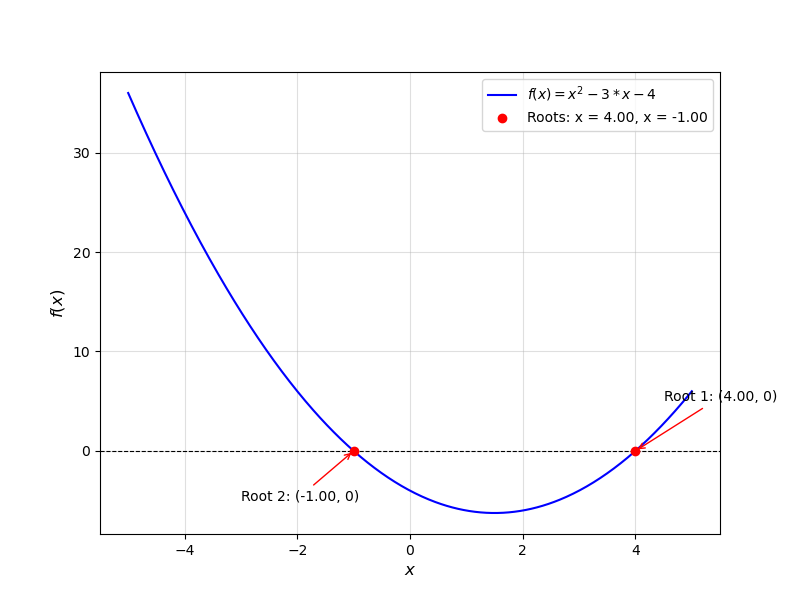
\includegraphics[width=1\columnwidth]{fig.png}
	\label{stemplot}
\end{figure}
    
\end{frame}
\end{document}
